\documentclass[12pt,twoside]{report}
\usepackage{tikz}
\usetikzlibrary{positioning, fit, arrows.meta}
\usepackage{amsmath,amssymb}

 
\usepackage{listings}
\usepackage{color}
 
\definecolor{codegreen}{rgb}{0,0.6,0}
\definecolor{codegray}{rgb}{0.5,0.5,0.5}
\definecolor{codepurple}{rgb}{0.58,0,0.82}
\definecolor{backcolour}{rgb}{0.95,0.95,0.92}
 
\lstdefinestyle{mystyle}{
    backgroundcolor=\color{backcolour},   
    commentstyle=\color{codegreen},
    keywordstyle=\color{magenta},
    numberstyle=\tiny\color{codegray},
    stringstyle=\color{codepurple},
    basicstyle=\ttfamily\footnotesize,
    breakatwhitespace=true,         
    breaklines=true,                 
    captionpos=b,                    
    keepspaces=true,                 
    numbers=left,                    
    numbersep=5pt,                  
    showspaces=false,                
    showstringspaces=false,
    showtabs=false,                  
    tabsize=2
}
 
\lstset{style=mystyle}

%%%%%%%%%%%%%%%%%%%%%%%%%%%%%%%%%%%%%%%%%%%%%%%%%%%%%%%%%%%%%%%%%%%%%%%%%%%%%

% Definitions for the title page
% Edit these to provide the correct information
% e.g. \newcommand{\reportauthor}{Timothy Kimber}

\newcommand{\reporttitle}{Chameleon Text: Exploring ways to increase variety in artificial data}
\newcommand{\reportauthor}{Thien P. Nguyen}
\newcommand{\supervisor}{Julia Ive, Lucia Specia}
\newcommand{\degreetype}{Computing (Machine Learning)}

%%%%%%%%%%%%%%%%%%%%%%%%%%%%%%%%%%%%%%%%%%%%%%%%%%%%%%%%%%%%%%%%%%%%%%%%%%%%%

% load some definitions and default packages
%%%%%%%%%%%%%%%%%%%%%%%%%%%%%%%%%%%%%%%%%
% University Assignment Title Page 
% LaTeX Template
% Version 1.0 (27/12/12)
%
% This template has been downloaded from:
% http://www.LaTeXTemplates.com
%
% Original author:
% WikiBooks (http://en.wikibooks.org/wiki/LaTeX/Title_Creation)
%
% License:
% CC BY-NC-SA 3.0 (http://creativecommons.org/licenses/by-nc-sa/3.0/)
% 
%
%%%%%%%%%%%%%%%%%%%%%%%%%%%%%%%%%%%%%%%%%
%----------------------------------------------------------------------------------------
%	PACKAGES AND OTHER DOCUMENT CONFIGURATIONS
%----------------------------------------------------------------------------------------
\usepackage[a4paper,hmargin=2.3cm,vmargin=2.0cm,includeheadfoot]{geometry}
\usepackage{textpos}
\usepackage{natbib} % for bibliography
\usepackage{tabularx,longtable,multirow,subfigure,caption}%hangcaption
\usepackage{fncylab} %formatting of labels
\usepackage{fancyhdr} % page layout
\usepackage{url} % URLs
\usepackage[english]{babel}
\usepackage{amsmath}
\usepackage{graphicx}
\usepackage{dsfont}
\usepackage{epstopdf} % automatically replace .eps with .pdf in graphics
\usepackage{backref} % needed for citations
\usepackage{array}
\usepackage{latexsym}
\usepackage[pdftex,pagebackref,hypertexnames=false,colorlinks]{hyperref} % provide links in pdf

\hypersetup{pdftitle={},
  pdfsubject={}, 
  pdfauthor={},
  pdfkeywords={}, 
  pdfstartview=FitH,
  pdfpagemode={UseOutlines},% None, FullScreen, UseOutlines
  bookmarksnumbered=true, bookmarksopen=true, colorlinks,
    citecolor=black,%
    filecolor=black,%
    linkcolor=black,%
    urlcolor=black}

\usepackage[all]{hypcap}


%\usepackage{color}
%\usepackage[tight,ugly]{units}
%\usepackage{float}
%\usepackage{tcolorbox}
%\usepackage[colorinlistoftodos]{todonotes}
% \usepackage{ntheorem}
% \theoremstyle{break}
% \newtheorem{lemma}{Lemma}
% \newtheorem{theorem}{Theorem}
% \newtheorem{remark}{Remark}
% \newtheorem{definition}{Definition}
% \newtheorem{proof}{Proof}


%%% Default fonts
\renewcommand*{\rmdefault}{bch}
\renewcommand*{\ttdefault}{cmtt}



%%% Default settings (page layout)
\setlength{\parindent}{0em}  % indentation of paragraph

\setlength{\headheight}{14.5pt}
\pagestyle{fancy}
\renewcommand{\chaptermark}[1]{\markboth{\chaptername\ \thechapter.\ #1}{}} 

\fancyfoot[ER,OL]{\sffamily\textbf{\thepage}}%Page no. in the left on odd pages and on right on even pages
\fancyfoot[OC,EC]{\sffamily }
\renewcommand{\headrulewidth}{0.1pt}
\renewcommand{\footrulewidth}{0.1pt}
\captionsetup{margin=10pt,font=small,labelfont=bf}


%--- chapter heading

\def\@makechapterhead#1{%
  \vspace*{10\p@}%
  {\parindent \z@ \raggedright \sffamily
    \interlinepenalty\@M
    \Huge\bfseries \thechapter \space\space #1\par\nobreak
    \vskip 30\p@
  }}

%---chapter heading for \chapter*  
\def\@makeschapterhead#1{%
  \vspace*{10\p@}%
  {\parindent \z@ \raggedright
    \sffamily
    \interlinepenalty\@M
    \Huge \bfseries  #1\par\nobreak
    \vskip 30\p@
  }}

\allowdisplaybreaks

% load some macros
% Here, you can define your own macros. Some examples are given below.

\newcommand{\R}[0]{\mathds{R}} % real numbers
\newcommand{\Z}[0]{\mathds{Z}} % integers
\newcommand{\N}[0]{\mathds{N}} % natural numbers
\newcommand{\C}[0]{\mathds{C}} % complex numbers
\renewcommand{\vec}[1]{{\boldsymbol{{#1}}}} % vector
\newcommand{\mat}[1]{{\boldsymbol{{#1}}}} % matrix


\date{May 2019}

\begin{document}

% load title page
% Last modification: 2015-08-17 (Marc Deisenroth)
\begin{titlepage}

\newcommand{\HRule}{\rule{\linewidth}{0.5mm}} % Defines a new command for the horizontal lines, change thickness here


%----------------------------------------------------------------------------------------
%	LOGO SECTION
%----------------------------------------------------------------------------------------


\includegraphics[width = 4cm]{./figures/imperial}\\[0.5cm] 

\center % Center remainder of the page

%----------------------------------------------------------------------------------------
%	HEADING SECTIONS
%----------------------------------------------------------------------------------------

\textsc{\Large Imperial College London}\\[0.5cm] 
\textsc{\large Department of Computing}\\[0.5cm] 

%----------------------------------------------------------------------------------------
%	TITLE SECTION
%----------------------------------------------------------------------------------------

\HRule \\[0.4cm]
{ \huge \bfseries \reporttitle}\\ % Title of your document
\HRule \\[1.5cm]
 
%----------------------------------------------------------------------------------------
%	AUTHOR SECTION
%----------------------------------------------------------------------------------------

\begin{minipage}{0.4\textwidth}
\begin{flushleft} \large
\emph{Author:}\\
\reportauthor % Your name
\end{flushleft}
\end{minipage}
~
\begin{minipage}{0.4\textwidth}
\begin{flushright} \large
\emph{Supervisor:} \\
\supervisor % Supervisor's Name
\end{flushright}
\end{minipage}\\[4cm]


%----------------------------------------------------------------------------------------
%	FOOTER & DATE SECTION
%----------------------------------------------------------------------------------------
\vfill % Fill the rest of the page with whitespace
Submitted in partial fulfillment of the requirements for the MSc degree in
\degreetype~of Imperial College London\\[0.5cm]

\makeatletter
\@date 
\makeatother


\end{titlepage}



% page numbering etc.
\pagenumbering{roman}
\clearpage{\pagestyle{empty}\cleardoublepage}
\setcounter{page}{1}
\pagestyle{fancy}

%%%%%%%%%%%%%%%%%%%%%%%%%%%%%%%%%%%%
% \begin{abstract}
% Your abstract.
% \end{abstract}

% \cleardoublepage
%%%%%%%%%%%%%%%%%%%%%%%%%%%%%%%%%%%%
% \section*{Acknowledgments}
% Comment this out if not needed.

% \clearpage{\pagestyle{empty}\cleardoublepage}

%%%%%%%%%%%%%%%%%%%%%%%%%%%%%%%%%%%%
%--- table of contents
\fancyhead[RE,LO]{\sffamily {Table of Contents}}
\tableofcontents 


% % \clearpage{\pagestyle{empty}\cleardoublepage}
\pagenumbering{arabic}
\setcounter{page}{1}
\fancyhead[LE,RO]{\slshape \rightmark}
\fancyhead[LO,RE]{\slshape \leftmark}

%%%%%%%%%%%%%%%%%%%%%%%%%%%%%%%%%%%%
% \chapter{Introduction}

% % \begin{figure}[tb]
% % \centering
% % 
\includegraphics[width = 0.4\hsize]{./figures/imperial}
% % \caption{Imperial College Logo. It's nice blue, and the font is quite stylish. But you can choose a different one if you don't like it.}
% % \label{fig:logo}
% % \end{figure}

% % Figure~\ref{fig:logo} is an example of a figure. 


% - Talk about the problem definition
% - talk about what you done
% - talk about the conclusion

%%%%%%%%%%%%%%%%%%%%%%%%%%%%%%%%%%%%

% So I would suggest go straight to the point: starting with describing the problem first, positioning it in the range of the related problems (as you mentioned yourself), introducing in details just the Seq2seq solution with some necessary background (as your baseline), mention the limitations of Seq2seq for your problem and ways they could be addressed (VAEs, etc.), describe the VAE approach and your motivation to pick it, introduce the VAE paper you work with in details.

%%%%%%%%%%%%%%%%%%%%%%%%%%%%%%%%%%%%
\chapter{Literature Survey}

\section{Artificial Data}

The premise of this literature survey is to describe the relevant components necessary to construct our solution, and to also discuss alternative approaches to the problem. 

% talk about the purpose:
% artificial data for NLP problems.
% why? lack of resources. datasets limited. unexplored.

\section{Text Generation}

% Text generation is a 

% - introduce the problem of text generation
% 	- large problem
% 	- lots of components
% 	- present solutions are relatively rudimentary in terms of their throughput.

% - we want to increase the lexical variety of the generated texts.
% 	- why? because we want to create data that looks similar to the original data, so we can use it as interim to other organisations that wish to request data. (That way, we don't reveal the original data in it's entirety.)

% - talk about the fact that this is an understudied problem; the described tools are commonly used in other areas of contempoary computer science.

Text generation is a a type of Language Modeling problem, which in itself, is one of the core natural language processing problems. It is used in a variety of contemporary applications, ranging from machine translation, to email response generation, to document summarisation.

In our particular case we imagine a scenario where a client requests the use of our dataset. We could permit them access to said data, but it would reveal the identities of the users in the data. The objective is to have some alternative dataset to ours such that value can be deduced from the data, but the privacy of the users in our original dataset is maintained.

This can be accomplished by creating a language model that would encompass the lexical variety of our original dataset. This language model would train on our original dataset, and would produce data that is semantically and lexically similar to our original data, but diverges enough such that it could potentially be seen as an entirely new and independent dataset. This new dataset can be assigned to other clients.

% problematics of controllable text generation?
% need to choose responses that are representative of the input, artificially.

\section{Language Modelling}

% Language modelling is the task of predicting the next word in a text given the previous words. It is probably the simplest language processing task with concrete practical applications such as intelligent keyboards and email response suggestion (Kannan et al., 2016)
Language modelling is the task of predicting a word $w_i$ in a text $w$ given some sequence of previous words $(w_1, w_2, ..., w_{i-1})$. More formally, \cite{dyer_conditional_2017} describes an unconditional language model as assigning a probability to a sequence of words,  $w = (w_1, w_2, ..., w_{i-1})$. This probability can be decomposed using the chain rule:

\begin{align}
p(w) = &{} p(w_1) \times p(w_2|w_1) \times p(w_3|w_1, w_2) \times ... \times p(w_i|w_1, w_2, ..., w_{i-1}) \\
p(w) = &{} \prod^{|w|}_{t=1}p(w_t|w_1, ..., w_{t-1})
\end{align}

Traditionally, assigning words to probabilities may conflate syntactically dubious sentences but it remains to be a useful method for representing texts.  

This paper concentrates on conditional language modelling. A conditional language model assigns probabilities to sequences of words, $w = (w_1, w_2, ..., w_{i-1})$, given a conditioning variable, $x$. 

\begin{align}
	p(\boldmath{w}|x) = &{} \prod^{|w|}_{t=1}p(w_t|x,w_1, ..., w_{t-1})
\end{align}

There exists different types of language models; we start with the n-gram, argued as being the most fundamental (\cite{le_recurrent_2018}). An n-gram is a chunk of n consecutive words in a sequential order. For instance, given the sentence "the quick brown fox \ldots", the respective n-grams are: 

\begin{itemize}  
	\item unigrams: "the", "quick", "brown", "fox"
	\item bigrams: "the quick", "quick brown", "brown fox"
	\item trigrams: "the quick brown", "quick brown fox"
	\item 4-grams: "the quick brown fox"
\end{itemize}

The intuition of n-grams was that statistical inference can be applied on the frequency and distribution of of the n-grams, which could be used to predict the next word. However, sparsity is not captured.

Later on, modern language models revolve around the use of neural networks (\cite{bengio_neural_2001}), which itself started off with a relatively modest MLP that formed the premise of word prediction. The use of neural networks in language modelling is often called Neural Language Modelling, of NLM for short.

Neural Networks are non-linear and computational metaphors of the brain that model arbitary relationships between input and output vectors. (This type of neural network architecture is commonly described as the multi-layer perceptron). Note that the input and output vectors are of a fixed dimension, which becomes a problem for our task at hand. Neural Networks evaluate an input using forward propagation, to produce an output. Traditionally, neural networks are trained to produce optimal outputs via the use of backpropagation. 

% something on neural language models being popular.

\section{Recurrent Neural Networks}
\label{rnn}
Recurrent neural networks (RNNs) are a class of feed forward neural networks such that the outputs are not necessarily restricted and discrete (as opposed to the MLP). RNNs operate over a sequence of variable-length vectors, and produces an output of similarly variable-length vectors. This circumvents a problem introduced with using an MLP, where sentences are not typically fixed length. 

The architecture of RNNs make it favourable in NLP related problems as words in sentences are typically conditioned on the previous words. When treated as language models, a standard RNN language model predicts each word of a sentence conditioned on the previous word and an evolving hidden state.

At each time step $t$, a simple RNN takes produces a hidden vector $h_t$, derived from the input vector $x_t$ and the previous state $h_{t-1}$ in the function $h_t = f_w(h_{t-1}, x_t)$. The hidden vector is usually obtained by some affine transformation offset by a bias vector, described in more detail in equation \ref{eq:rnn}. The same function and the same parameters are used at each time step $t$. RNNs typically are not parallelised. 

\begin{equation}
	\label{eq:rnn}
	\begin{aligned}
		h_t &= tanh(W_{hh}h_{t-1}+W_{xh}x_t)
	\\
	y_t &= W_{hy}h_t
	\end{aligned}
	\end{equation}

RNNs are typically trained with backpropagation through time. The gradient flow $w \leftarrow w - \alpha ({\delta L}/{\delta w})$ is computed at every timestep, meaning that every path from $W$ to the loss $\mathcal{L}$ needs to be considered.

\begin{equation}
	\label{eq:btt}
	\begin{aligned}
		\frac{\delta L}{\delta w} = \sum^T_{j=0}\sum^j_{k=1}\frac{\delta L_j}{\delta y_j}\frac{\delta y_j}{\delta h_j}(\prod^j_{t=k+1}\frac{\delta h_t}{\delta h_{t-1}})\frac{\delta h_k}{\delta w}
	\end{aligned}
	\end{equation}


Typically, there are two caveats with training RNNs. One of which involves the sensitivity of the gradients: The product symbol within the loss function in \ref{eq:btt} is the cause of vanishing and exploding gradients. The sensitivity of the gradients make it especially difficult to train RNNs. 
Additionally, it became aparrent that it was very difficult for RNNs to leverage relationships between potentially relevant inputs and outputs - there isn't necessarily a clear indicator in the architecture that would facilitate this feature. This is described as a long range dependency problem.

\subsection{LSTMs and GRUs} 

Both gates were introduced to circumvent the issue of long range dependency problems by providing multiple avenues, with each one having a different approach.

\begin{figure}[!ht]
\begin{equation}
  \begin{split}
    i_t &= \sigma(W_i \cdot [h_{t-1},x_t] + b_i) \\
    f_t &= \sigma(W_f \cdot [h_{t-1},x_t] + b_f) \\
		o_t &= \sigma(W_o \cdot [h_{t-1},x_t] + b_o) \\
		g_t &= \sigma(W_g \cdot [h_{t-1},x_t] + b_g) \\
		c_t &= f_t \odot c_{t-1} + i_t \odot g_t \\
		h_t &= o_t \odot tanh(c_t) 
  \end{split}
% \quad\leftrightarrow\quad
	\quad\quad
  \begin{split}
		u_t &= \sigma(W_u \cdot [h_{t-1},x_t] + b_u) \\
		r_t &= \sigma(W_r \cdot [h_{t-1},x_t] + b_r) \\
		c_t &= tanh(Ww_{t-1}+U(r_t \odot h_{t-1})) \\
		h_t &= (1-u_{t})\odot h_{t-1} + u_t \odot c_t
  \end{split}
\end{equation}
\caption{Equations for LSTM cells (left) and GRU cells (right).}
\end{figure}
 
LSTM (Long Short Term Memory; \cite{hochreiter_long_1997}) are a type of RNN cell that attempts to retain information based on the previous inputs through the introduction of gated architectures. 

GRUs (Gated Recurrent Units; \cite{cho_properties_2014}) are functionally similar to LSTMs, but uses less parameters. Within the GRU architecture, a feature to retain the previous weights remain, but there exists an direct path to the input data from the output, allowing a reduction in training time. They are unable to clearly distinguish between the performance of the two gated units they tested. \cite{chung_empirical_2014} suggests that GRUs were found to perform at least equivalent to LSTMs but show slight improvements on smaller datasets. 

\section{Autoencoders}

% need citation
Autoencoders are a specialised form of neural networks where the model attempts to recreate the inputs on the output. Autoencoders typically have  layer in the model where its dimension is smaller than the input space, therefore representing a dimensionality reduction in the data. 
% need reference to PCA

Autoencoders are composed of two different principal components, an encoder network $\alpha$ and a decoder network $\beta$, such that $\alpha : X \rightarrow F$ and $\beta : F \rightarrow X$. Measuring the success of the reconstruction is deduced by a reconstruction loss formula. This reconstruction loss comapres the output of the decoder and compares it against the input of the encoder. The two networks are trained together in a manner that allows them to preserve the input as much as possible.
% definitely need a diagram for autoencoders
% what is it good for?

% talk about how hard it is to understand the structure of the latent variable and how this prevents us from sampling.

Autoencoders are popularised through their use in Machine Translation, Word Embeddings, and document clustering. 

% talk about how important this is in the context of the task.
\subsection{Variational Autoencoders}

Variational Autoencoders (VAEs, \cite{kingma_auto-encoding_2013}) are based on a regularised version of the standard auteoncoder. VAEs forces the encoder to learn parameters of a gaussian distribution - a mean and a covariance - as opposed to creating a fixed latent vector. In more discrete terms, it replaces the encoder from the standard autoencoder with a learned posterior \textit{recognition model}, $q(\overrightarrow{z}|x)$. This component of the autoencoder parameterises an approximate posterior distribution over $\overrightarrow{z}$, using a neural network conditioned on $x$. This consequently allows us to take advantage of recent advances in variational inference.  A sample is taken from a gaussian using the learned parameters, which is then fed into the decoder. Training this particular model involves learning the parameters involved for our latent distribution.

\begin{figure}[!ht]
	\centering
	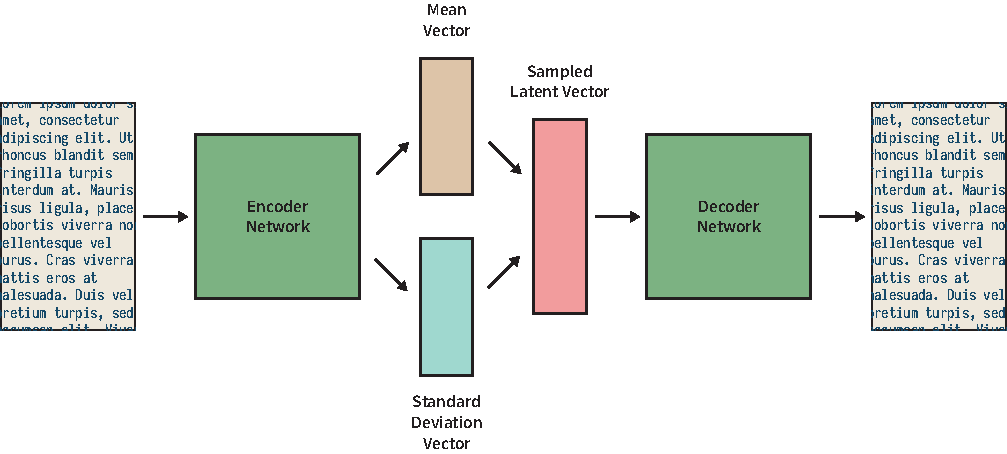
\includegraphics[width=150mm]{diagrams/variational_autoencoders.pdf}
	\caption{An abstracted model architecture for a variational autoencoder, which takes as input some text, and it's predicted output being the same text as the input.\label{vae}}
  \end{figure}

Note that the decoder receives samples from a non-standard normal distribution produced by the encoder. The average of the samples of the different distributions should approximate to a standard normal. This stochasticity allows us to model variability in the results. 

If VAEs were trained with a standard autoencoder's reconstruction objective, then it would learn to encode it's inputs determinsitically by making variances in \textit{recognition model}, $q(\overrightarrow{z}|x)$ vanishingly small. (\cite{raiko_techniques_2014}) Instead, the loss function for VAEs is composed of two components; a reconstruction loss that involves an expection of the output; and a KL divergence (see Equation \ref{eqn:kl_divergence}), which measures the distribution of the posterior distributions against a standard gaussian $ \mathcal{N}(0,1)$). This objective provides a valid lowerbound on the true likelihood of the data, making VAEs a generative model.
  
\begin{equation}
	\label{eqn:elbo}
	\mathcal{L}(\theta, \phi, x, z) = \mathbb{E}_{q \phi (z|x)}[log \thinspace p_{\theta}(x|z)] - D_{KL}(q_{\phi}(z|x)\thinspace||\thinspace p(z)) \leq log (p(x))
\end{equation}

\begin{equation}
	\label{eqn:kl_divergence}
D_{KL}(P ||Q) = \sum_{x \subset X} P(x) \cdot log (\frac{P(x)}{Q(x)})
\end{equation}
In other words, it is the expectation of the logarithmic difference between the probabilities $P$ and $Q$, where the expectation of $P$ is already known.

\subsubsection*{Reparameterisation Trick}

$$z = \mathcal{N}(\mu, \Sigma) \equiv \mu + \Sigma \cdot \epsilon $$ 


The Gaussian reparameterisation trick (\cite{kingma_auto-encoding_2013}) subverts the issue of performing backpropagation against sampled latent variables through the rearrangement of the gaussian parameters. Instead of sampling $z$ through a gaussian $\mathcal{N}(\mu, \Sigma)$, $z$ can be created by a summation of $\mu$ and some gaussian noise $\epsilon \sim \mathcal{N}(0,1)$ applied to $\Sigma$. This rearrangement allows for derivatives to be calculated with respect to the parameters that are needed for learning.


\subsection{Conditional Variational Autoencoders}

In a VAE, the decoder class cannot produce outputs of a particular class on demand. CVAEs are an improved model of the original VAE architecture by conditioning on another description of the data, a class descriptor $y$. 

\begin{figure}[!ht]
      
	\centering
	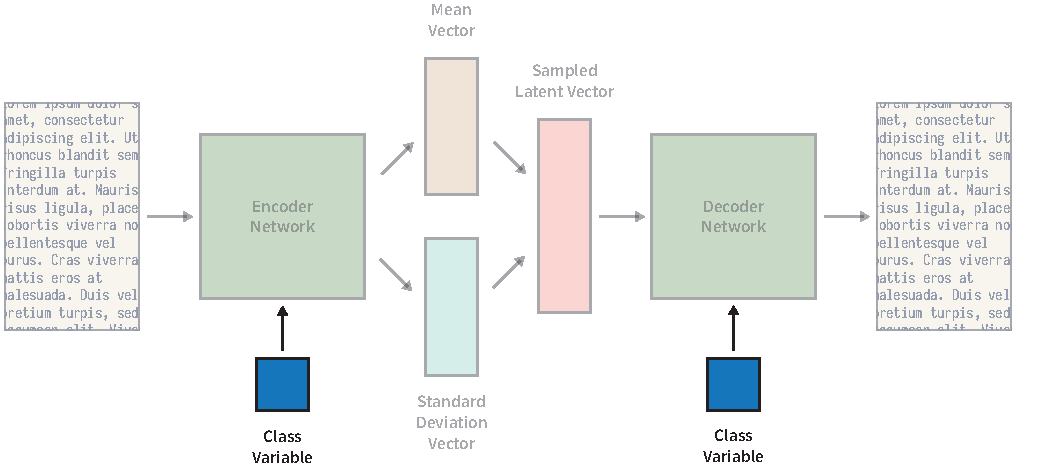
\includegraphics[width=150mm]{diagrams/conditional_variational_autoencoders.pdf}
	\caption{A model architecture for a CVAE, which includes the label being fed into the encoder and decoder networks. \label{cvae_diagram}}
  \end{figure}

During training time, a class (represented by some arbitary vector) is fed at the same time to the encoder and decoder. To generate an output that depends on $y$ we feed that number to the decoder along with a random point in the latent space sampled from a standard normal distribution.

Samples can be generated from the conditional distribution $p(x|y)$. By changing the value of $y$, we can get corresponding samples $x \sim p(x|y)$. The system no longer relies on the latent space to encode what output is necessary; instead the latent space encodes other information that can distinguish itself based on the differing $y$ values.

% However, it was found by \cite{du_variational_2018} that since the responses were generated from the same latent variable (induced by the class), it was difficult to model high-variability in responses.

% That being said, using this model alone is not sufficent. If we train the dataset on a vanilla VAE, assuming that the dataset can be encapsulated and modelled in such a manner that allows it to be processed in the model, outputs from the VAE alone will only produce some latent representive of the mean of the training data. 

In terms of implementation, it happens to be more feasible to concate the class variable to the dataset prior to feeding. This allows the model to retain its characteristics without needing to adjust in order to accomadate the conditioning variables.


\section{Related Work}

\subsection{Sequence To Sequence}

Sequence to Sequence, (seq2seq, \cite{sutskever_sequence_2014}) is a type of neural language model that models relationships between sequences. In our particular scenario, this could be seen as a modern interpretation of the autoencoder. Seq2Seq comprises of two components, encoders and decoders, both of which are represented with RNN models (although can be replaced with LSTM or GRU cells). The last hidden state value of the encoder is recognised as the context variable, which encodes the characteristics of the input sequence. This is used as the first hidden vector value for the decoder. 

\begin{figure}[!ht]
		
\centering
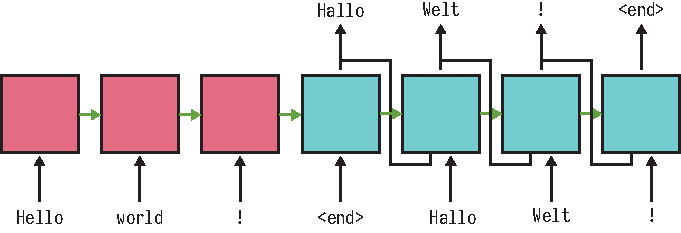
\includegraphics[width=100mm]{diagrams/seq2seq.pdf}
\caption{An abstracted model of the seq2seq architecture, where the encoder (pink) takes in the input sequence, and the decoder (blue) shows the output sequence.\label{seq2seq}}
\end{figure}

Seq2seq models have shown to be effective in reponse generation, but is no longer considered to be state of the art. For instance, the context variable itself is considered to be bottlenecked as it has to encompass the entire input sequence in a single vector. As we've discussed earlier in Section \ref{rnn}, the training mechanism is subject to vanishing and exploding gradients; it becomes increasingly difficult to retain information about earlier parts of the sequence as opposed to recent parts of the sequence in the encoder stages as a consequence. We explain later about approaches to mitigate the issue.

Furthermore, the responses produced from a vanilla seq2seq model tends to lack lexical diversity and richness (\cite{serban_hierarchical_2016}, \cite{zhao_learning_2017}, \cite{jiang_why_2018}). There tends to be many causes, but one reason (which we tackle in the paper) is due to the lack of statistical inferencing. The model itself lacks the possibilty of presenting a variety of lexical responses in the decoder, in a manner that a VAE could.

\subsubsection{Variational Context}

\begin{figure}[!ht]
	\centering
	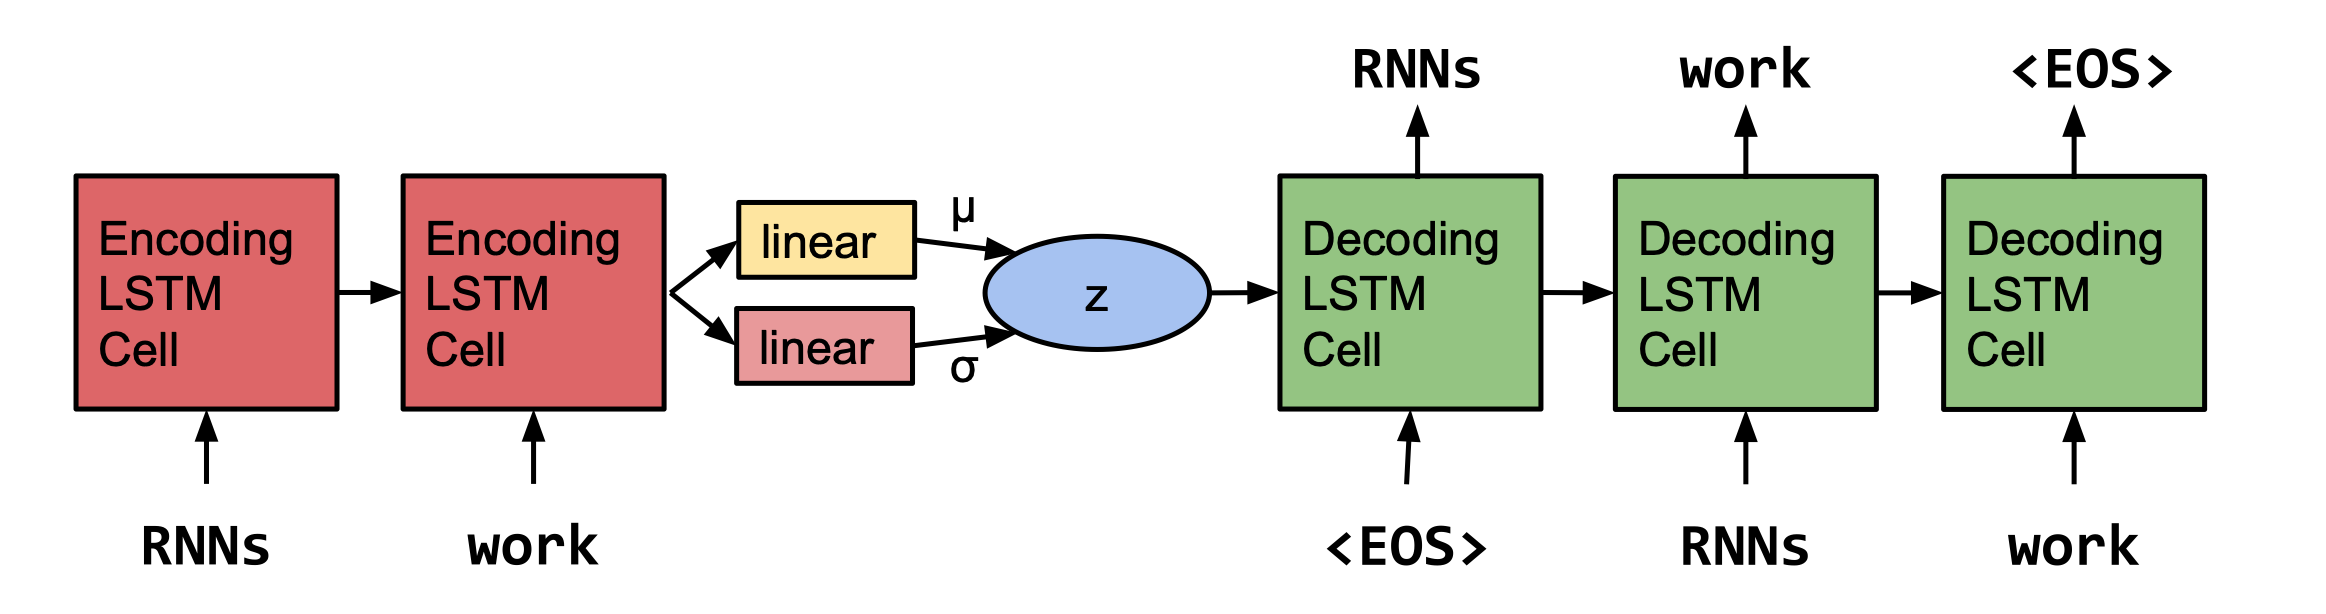
\includegraphics[width=100mm]{diagrams/seq2seqvae.png}
	\caption{The core structure of the VAE language model - words are represented as embedded vectors (\cite{bowman_generating_2015}). \label{seq2seq_attn}}
\end{figure}

Instead of passing through the last hidden state drom the encoder to the decoder, it is possible to encode the context variable produced from the encoder in the form of gaussian parameters in a similar fashion to how VAEs are designed (\cite{bowman_generating_2015}).  

The model is trained in a similar fashion to VAEs in general (see Equation \ref{eqn:elbo}) but utilises additional mechanisms to force the language model to encode features into the gaussian parameters. We explain these features in further detail in Section \ref{optimisation_challenges}.

\subsubsection{Attention Mechanisms}

\begin{figure}[!ht]
      
	\centering
	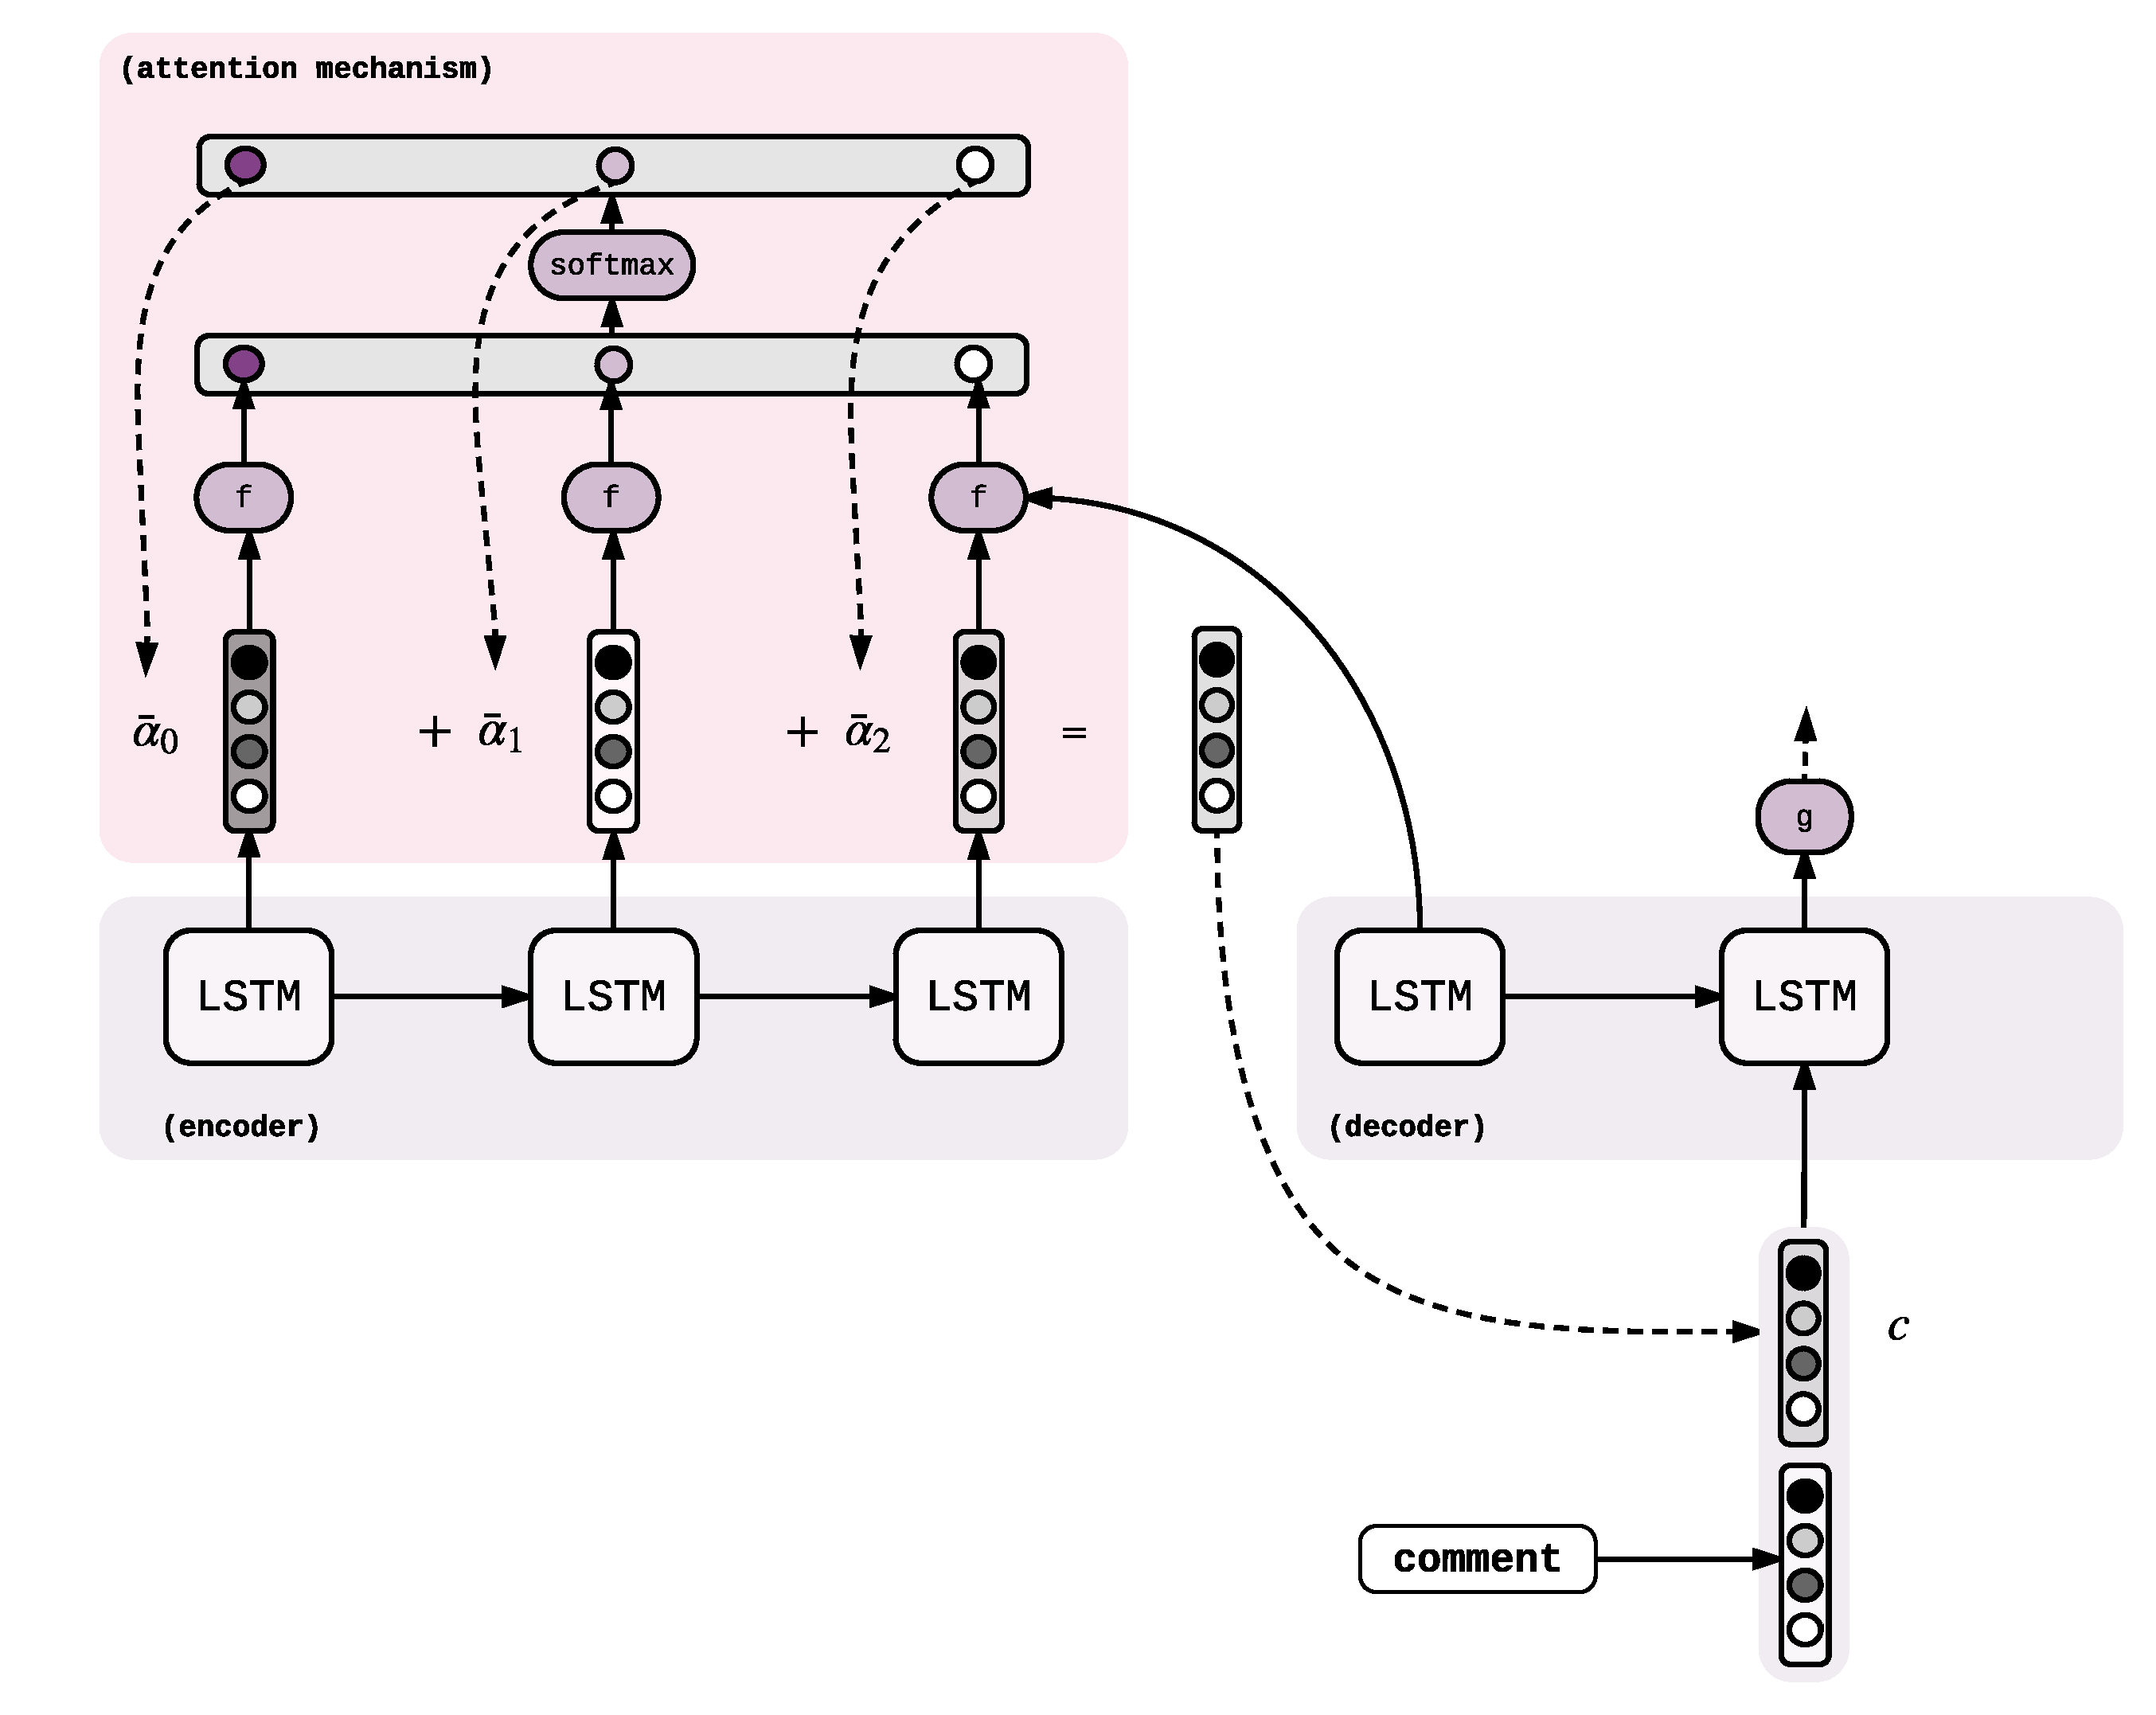
\includegraphics[width=100mm]{diagrams/seq2seq_attention_mechanism.pdf}
	\caption{An abstracted diagram of the attention mechanism, applied to a seq2seq model.\label{seq2seq_attn}}
\end{figure}
% https://guillaumegenthial.github.io/sequence-to-sequence.html

In addition to the context vector, the decoder can also retrieve information on the encoder values using attention (\cite{bahdanau_neural_2014}). This mechanism looks at all of the inputs from the hidden states of the encoders so far. This allows the decoder network to "attend" to different parts of the source input at each step of the output generation. This circumvents the need to encode the full source input into a fixed-length vector, helping it deal with long-range dependency problems.

% fix this section
Furthermore, this attention mechanism allows the model to learn what to attend to based on the input sequence and what it has so far, represented through a weighted combination of the two.

Attention mechanisms were found to perform particularly well in machine translation problems where languages which are relatively well aligned (such as English and German). The decoder is most likely able to choose to attend to the response generation sequentially, such that the first output from the decoder can be generated based on the properties of the first input of the encoder and so on.

% mention the limitations of Seq2seq for your problem and ways they could be addressed (VAEs, etc.), describe the VAE approach and your motivation to pick it, introduce the VAE paper you work with in details.

% \subsection{Transformers}

% \begin{figure}[!ht]
      
% 	\centering
% 	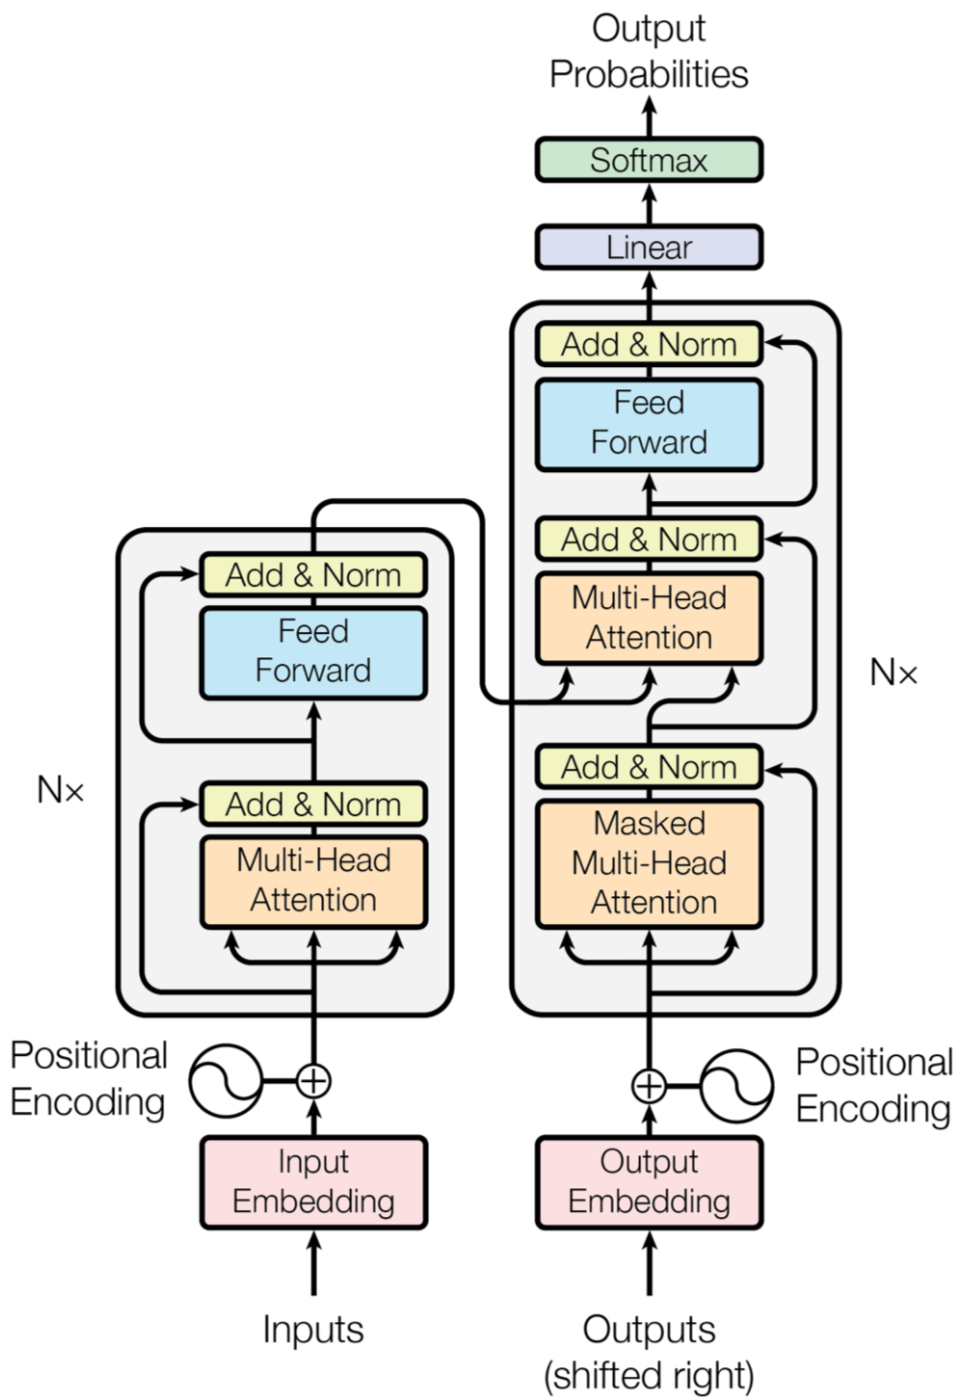
\includegraphics[width=60mm]{diagrams/transformers.png}
% 	\caption{The transformer model architecture.\cite{vaswani_attention_2017} \label{transformer}}
%   \end{figure}

% Transformers (\cite{vaswani_attention_2017}) are a neural language model that avoids the use of RNNs altogether and focuses on using solely the attention mechanism (\cite{bahdanau_neural_2014}). The model consequently  utilises stacked layers of residual networks for the encoder and the decoder that encodes attentive properties of the input, described as self attention heads. This shift in architecture affords improvements to computational throughput, and can also be computed in parallel.

% \subsubsection{Self Attention}

% \begin{align}
% \label{eqn:eqlabel}
% \begin{split}
% 	Q = X \cdot W^Q \\
% 	K = X \cdot W^K \\
% 	V = X \cdot W^V 
% \end{split}
% \end{align}

% Self attention mechanisms involve three components, a Query $Q$, Key $K$, and Value $V$. 

% \begin{equation}
% 	z = \sigma(\frac{Q \cdot K^T}{\sqrt{d_k}})\cdot V
% \end{equation}

% The product of multiple $z$ variables concatenated together, with a weights matrix $W^O$ a multihead attention $\boldsymbol{z}' = \lbrack z_1,...,z_n \rbrack \cdot W^O$. 

% \begin{equation}
% 	\boldsymbol{r} = f_{NN}(\boldsymbol{z})
% \end{equation}

% \subsubsection{Positionality Hack}

% Sequential models circumvent the referential ambiguity problems with natural language (such as "the cat is on the mat"), with the inherent properties of time based encodings. This does not necessarily translate well to encoder models as there is no sequentiality. To circumvent this, Transformers encode the positions of words at the embedding level, by adding positional encodings of words.

% %%%%%%%%%%%%%%%%%%%%%%%%%%%%%%%%%%%%


\chapter{Model}

In this chapter we discuss the current implementation in detail. It builds on the knowledge in the first chapter, and the model itself is a combination of features described above.

\section{Variational Autoregressive Decoders}

To increase variability of outcomes produced by the original seq2seq model, \cite{serban_hierarchical_2016}; \cite{zhao_learning_2017} proposed the use of variational autoencoders to seq2seq models. At generation time, the latent variable $z$ can be used as a conditional signal of the decoder in the seq2seq model. Although this introduces variability in the outputs, the variability is not controlled; i.e it is produced from the randomness of $z$. The underlying seq2seq model remains suboptimal.

Introduced by \cite{du_variational_2018}, Variational Autoregressive Decoders (VADs) attempt to circumvent the sampling problem introduced from CVAEs by introducing multiple latent variables into the autoregressive Decoder. At different time-steps, this allows the decoder to produce a multimodal distribution of text sequences, allowing a variety of responses to be produced. 

We will be using this model to help solve the variability of outcomes. *WHY?*

VADs use the seq2seq architecture as the base with variable-length queries $x = \{x_1, x_2, ..., x_n\}$, and $y = \{y_1, y_2, ..., y_n\}$ representing the input and output responses respectively. The encoder network is a Bidirectional RNN with GRUs. The decoder network is an unidirectional RNN with GRUs. For each timestep $t$, each GRU in the decoder network is encoded with hidden state $h^d_t$.

% need a diagram

\subsubsection{Encoder}

\begin{align}
\label{eqn:eqlabel}
\begin{split}
	\overrightarrow{h^e_t} = \overrightarrow{GRU}(x_t, \overrightarrow{h^e_{t-1}})
\\
\overleftarrow{h^e_t} = \overleftarrow{GRU}(x_t, \overleftarrow{h^e_{t+1}})
\end{split}
\end{align}

The encoder works in a similar fashion to the encoder described in the seq2seq network. The only changes here we see is that the encoder described in the implementation leverages bi-directionality. This leverages the sequentiality of the sequence in both directions (left to right, and vice versa.) This is made possible by stacking two recurrent cells on top of each other. 

\subsubsection{Backwards}

\begin{align}
\label{eqn:eqback}
\overleftarrow{h^d_t} = \overleftarrow{GRU}(y_{t+1}, \overleftarrow{h^d_{t+1}})
\end{align}

The backwards RNN is one of the components used to condition the latent variable $z$ in the decoder. During training, the backwards RNN takes as input the training outputs $y$ and outputs hidden vectors in a sequential manner.

\subsubsection{Attention}

\begin{equation}
\label{eq:attn}
\begin{aligned}
	\alpha_{s,t} &= f_{attention}([h^e_d, h^d_{t-1}])\\        
	c_t &= \sum^m_{s=1}\alpha_{s,t} h^e_s
\end{aligned}
\end{equation}

- Uses Luong's Attention mechanism that involves a concatenation.
- uses a backwards RNN that represents the actual response to better create a posterior distribution.

\subsubsection{Inference Model}

\begin{equation}
\label{eq:t}
\begin{aligned}
\lbrack \mu^i, \sigma^i \rbrack &=
f_{infer}([\overrightarrow{h^d_{t-1}}, c_t, \overleftarrow{h^d_t}])
\\
q_{\theta}(z_t|\boldsymbol{y}, \boldsymbol{x}) &= \mathcal{N}(\mu^i, \sigma^i)
\end{aligned}
\end{equation}

The inference model attempts to create a posterior distribution $z$ using the conditioned output, the attention weights, and the decoder outputs.

\subsubsection{Prior Model}

\begin{equation}
\label{eq:t}
\begin{aligned}
\lbrack \mu^p, \sigma^p \rbrack &=
f_{infer}([\overrightarrow{h^d_{t-1}}, c_t])
\\
p_{\phi}(z_t|\boldsymbol{y}_{<t}, \boldsymbol{x}) &= \mathcal{N}(\mu^p, \sigma^p)
\end{aligned}
\end{equation}

The prior network is restricted to using observable variables in the testing phase in order to generate $z_t$. It is designed in a similar fashion to the decoder network where the input variables are concatenated together.

\subsubsection{Decoder (Variational Autoregressive)}

\begin{equation}
	\overrightarrow{h^d_t} = \overrightarrow{GRU}([y_{t-1},c_t,z_t], \overrightarrow{h^d_{t-1}})
\end{equation}
\begin{equation}
	p_\phi(y|\boldsymbol{y}_{<t},\boldsymbol{z}_t, \boldsymbol{x}) = f_{output}([\overrightarrow{h^d_t}, c_t])
\end{equation}

This component stems away from \cite{zhao_learning_2017}, as $\boldsymbol{z}$ is now decomposed into sequential variables $\boldsymbol{z} = \{z_1,...,z_t\}$, which are generated at each time step of the decoder phase. $z_t$ is conditioned by the backwards hidden vector $h^d_{t}$. \cite{du_variational_2018} suggests that this conditioning allows the latent variables to be guided for long-term generation.

\subsubsection{Auxillary Objective}

An auxillary objective that attempts to predict the bag of words based on the latent variable. Helps to improve the output options. Let $f=MLP_b(z_t) \in \mathcal{R}^V$ where $V$ be the vocabulary size:

\begin{equation}
	log [p_\xi(y_{bow(t+1,T)}|z_{t:T}) ] = log  \frac{e^{f_{z_{t}}}}{\sum^V_j e^{f_{j}}}
\end{equation}

\subsubsection{Learning Mechanism}

VADs use a weighted combination of ELBO (Equation \ref{eqn:elbo})  the log likelihood loss of the auxillary objective.

\begin{equation}
	\mathcal{L}'(\theta, \phi, x, c) =\mathcal{L}'(\theta, \phi, x, c) + E_{q_{\phi}(z|c,x,y)}[log(p(x_{bow}|z,c))]
\end{equation}

\subsubsection{KL Divergence Derivation}

Let $\mu_1, \sigma_1 \rightarrow \mathcal{N}(\mu_1,\sigma_1)$ be our first distribution, and $\mu_2, \sigma_2 \rightarrow \mathcal{N}(\mu_2,\sigma_2)$ be our second distribution. By deriving this, we would be able to calculate a derivative friendly loss function for our models.

\begin{equation}
	\label{eq:t}
	\begin{aligned}
	KL &= \int \left[\log( p(x)) - \log( q(x)) \right]\ p(x)\ dx \\
	% &= \frac{1}{2}\left[\log\frac{|\Sigma_2|}{|\Sigma_1|} - d + tr(\Sigma_2^{-1}\Sigma_1) + (\mu_2 - \mu_1)^T \Sigma_2^{-1}(\mu_2 - \mu_1)\right] \\
	&= \int \left[ \frac{1}{2} \log\frac{|\Sigma_2|}{|\Sigma_1|} - \frac{1}{2} (x-\mu_1)^T\Sigma_1^{-1}(x-\mu_1) + \frac{1}{2} (x-\mu_2)^T\Sigma_2^{-1}(x-\mu_2) \right] \times p(x) dx \\
	&= \frac{1}{2} \log\frac{|\Sigma_2|}{|\Sigma_1|} - \frac{1}{2} \text{tr}\ \left\{E[(x - \mu_1)(x - \mu_1)^T] \ \Sigma_1^{-1} \right\} + \frac{1}{2} E[(x - \mu_2)^T \Sigma_2^{-1} (x - \mu_2)] \\
	&= \frac{1}{2} \log\frac{|\Sigma_2|}{|\Sigma_1|} - \frac{1}{2} \text{tr}\ \{I_d \} + \frac{1}{2} (\mu_1 - \mu_2)^T \Sigma_2^{-1} (\mu_1 - \mu_2) + \frac{1}{2} \text{tr} \{ \Sigma_2^{-1} \Sigma_1 \} \\
	&= \frac{1}{2}\left[\log\frac{|\Sigma_2|}{|\Sigma_1|} - d + \text{tr} \{ \Sigma_2^{-1}\Sigma_1 \} + (\mu_2 - \mu_1)^T \Sigma_2^{-1}(\mu_2 - \mu_1)\right].
\end{aligned}
\end{equation}

We derive the KL Divergence as we no longer measure the distance of our posterior distribution against a standard gaussian. We instead train the 

% Although these models have been used in NMT related problems, sequence generation is often unexplored within NLP. We propose using models that traditionally perform well in NMT problems and adapt them for use with sequence generation problems. 

\section{Data Augmentation}

\begin{figure}[!ht]
\centering
\lstinputlisting[language=java]{dataset_1.txt}
\lstinputlisting[language=python]{dataset_2.txt}
\caption{A sample review and the augmented data. Note that for each sequence from line 3 onwards has the identity sequence contatenated before it. \label{aug_1}}
\end{figure}

The dataset produced has to be augmented in order for the model to process them. 

\subsection{Embeddings}

We use the glove word2vec word embeddings.

\subsection{Review Prepropressing}

The model would be forced to produce the next sentence from the previous sentence. Sentences are split by periods. Tokens are represented as words or individual punctuation marks. Additional tags are introduced. Lowercase. 

ASIN represents item ID. this is split by characters.

\subsection{Polarity Calculation}

This is calculated with:

\begin{equation}
p = \sigma_{tanh}(\frac{h_{pos} - h_{neg}}{h_{pos} + h_{neg}})
\end{equation}

The polarity word vector is a sum of the polarity value $p$ and the word vector corresponding to the word "polarity".

\subsection{Implementation}

Built on PyTorch. Models take a considerable amount of time to train, which does not necessarily align with rapid evolution of the implementation. Components are typically built with states in mind such that when running a model, it keeps a state of the source codes at the time of running in its own results container. This allows us to repeat the results using the code produced at the time.

\subsubsection{Weight Initialisation}

Typically, we start with wanting to have the weights being asymmetric (such that when we perform our gradient descent we would have random starting positions, which would enable us to have a better chance to find the minimum as opposed to having a fixed starting point). Fortunately, pulling from a gaussian distribution is sufficent. The problem here is that we're fixing some parameter for the standard deviation. 

% Xavier [Glorot et al.](http://proceedings.mlr.press/v9/glorot10a/glorot10a.pdf)

Xavier 
proposed to initialise the weights based on a gaussian $Var(w)=\mathcal{N}(0,\frac{2}{|n_{in}| + |n_{out}| })$ where $w$ represents a layer in a network, and $|n_{in}|$ represents the number of neurons feeding into it, and similarly so for $|n_{out}|$. Note that I have used a gaussian distribution, but it can also be uniform. This method has shown a lot of success for sigmoid and tanh based activation functions.

For ReLU based networks, 
% [Kaiming et al.](https://arxiv.org/pdf/1502.01852.pdf) 
suggests that the weights should be initialised using $Var(w)=\mathcal{N}(0,\frac{2}{|n_{in}|})$. 

\section{Optimisation Challenges}
\label{optimisation_challenges}

In addition to the fact that RNNs itself are difficult to train (see Section \ref{rnn}), it is commonly the case that the latent variable is often ignored during training.

Ideally, a model that encodes useful information in the latent variable $\overrightarrow{z}$ will have a non-zero KL divergence term and a relatively small cross-entropy term. Straightforward implementations of our model failed to learn this behaviour.

Due to the sensitivity of our model, which is compounded by the sensitivity of the GRU cells in our model, early implementations of our model would initially ignore $\overrightarrow{z}$ and go after the low hanging fruit during the learning process of the decoder. Once this occurs, the decoder ignores the encoder and gradients between the two components become non-existent, preventing learning.

is it often likely that in a degenerative setting, the latent vector in the model would encorporate a lack of relevant information and is essentially ignored. This results in a KL collapse s.t the KL loss reaches zero, and thus the model is then effectively equivalent to an RNN language model.

\subsection{Teacher Forcing}

Teacher Forcing (\cite{williams_learning_1989}) is a concept of using real target outputs as each next input in the decoder sequence as opposed to using the decoder's guess. This causes the model to converge faster, but may exhibit instability when the trained network is exploited.

Outputs can be observed when using teacher forced decoders that read with coherent grammar but can wander far from the correct response. Typically, this can be controlled with a probability $p$ such that the decoder sequence has a $p$ chance of using teacher forcing during training.

\subsection{KL Annealing}

A simple approach by \cite{bowman_generating_2015}, it involves adding a variable weight to the KL term in the cost function at training time. Initially, the weight is zero, forcing the model to encode as much information into the latent variable as much as it can. The weight is then gradually increased, eventually reaching 1. At this stage the weighted cost function is equivalent to the ELBO loss. This could be thought of as annealing from a regular autoencoder towards a variational one.

\subsection{Word Dropout}
Also proposed by \cite{bowman_generating_2015}, it involves weakening the decoder by removing some conditioning information during training. This is done by randomly replacing a fraction of the conditioned-on word tokens with a generic unknown token UNK, which forces the model to depend on the latent variable $z$ for prediction. This works in a similar fashion to the standard dropout (\cite{srivastava_dropout:_2014}) where connections are dropped between layers of a network, but is applied to the input data of a recurrent cell.

\section{Testing Method}

We benchmark the performance of our model against a regular seq2seq network, alongside a transformer. 

The objective is to 

her the data produced corresponds to a fake model or from the dataset. This is not used as a loss function (this would consequently create a generative model).

We compare the performance of the VAD against two baselines, a seq2seq model described above and the Transformer.

Models are computed on an 4.4GHz intel 3770k with a GTX 1080 with 8GB VRAM.


\subsection{Measuring Performance}

To understand the quality of our models, we subject them to BLEU (\cite{papineni_bleu:_2001}) and ROUGE (\cite{lin_rouge:_2004}) scores at each epoch to measure the quality of our responses. These measurements are used alongside the Loss, which will measure the rate of learning.



BLEU (\cite{papineni_bleu:_2001}) is originally defined with $n$-gram precision $p_n$ by summing the $n$-gram matches for every hypothesis sentence $S$ in the test corpus $C$. In our particular case, we use unigrams.

\begin{figure}[!ht]
	\begin{equation}
		\begin{split}
			p_n = \frac
			{\sum_{S\in C} \sum_{ngram\in S} Count_{clip}(ngram)}
			{\sum_{S\in C} \sum_{ngram\in S} Count(ngram)}
		\end{split}
	% \quad\leftrightarrow\quad
		\quad\quad
		\begin{split}
			p_n = \frac
			{\sum_{S\in C} \sum_{ngram\in S} Count_{matched}(ngram)}
			{\sum_{S\in C} \sum_{ngram\in S} Count(ngram)}
		\end{split}
	\end{equation}
	\caption{Equations for BLEU (left) and ROUGE  (right).}
	\end{figure}

% https://stackoverflow.com/questions/38045290/text-summarization-evaluation-bleu-vs-rouge

Although both equations look very similar, BLEU  BLEU introduces a brevity penalty term, and also compute the n-gram match for several size of n-grams (unlike the ROUGE-n, where there is only one chosen n-gram size). 

"Bleu measures precision: how much the words (and/or n-grams) in the machine generated summaries appeared in the human reference summaries.

Rouge measures recall: how much the words (and/or n-grams) in the human reference summaries appeared in the machine generated summaries.

Naturally - these results are complementing, as is often the case in precision vs recall. If you have many words from the system results appearing in the human references you will have high Bleu, and if you have many words from the human references appearing in the system results you will have high Rouge."


% http://opennmt.net OPENMNT-Py has BLEU/ROUGE on it.

% %%%%%%%%%%%%%%%%%%%%%%%%%%%%%%%%%%%%
% \chapter{Experimental Results}

% \chapter{Future Work}

% %%%%%%%%%%%%%%%%%%%%%%%%%%%%%%%%%%%%
% \chapter{Conclusion}


%% bibliography
\bibliographystyle{apa}
\bibliography{ref} 

\end{document}
